\section[Proiectarea unui divizor de tensiune]{Proiectarea unui divizor de tensiune (facultativ)}

'In sec'tiunea \ref{subsection:ca_sisteme} (Fig. \ref{fig:divizor_tensiune_gol_sistem}) am considerat divizorul de tensiune ca un sistem, 'in care (tensiunea de) ie'sire depinde de (tensiunea de) intrare prin func'tia de transfer $H = \frac{1}{1+\alpha}$, unde $\alpha = \frac{R_1}{R_2}$ reprezint'a raportul 'intre rezistoarele ${R_1}$ 'si $R_2$. 

Astfel, pare c'a modul de comportare a circuitului este determinat doar de acest raport $\alpha$, rezisten'tele ${R_1}$ 'si $R_2$ put\^and lua orice valoare, at\^ata timp c\^at se p'astreaz'a raportul dintre ele. 

'In realitate lucrurile sunt 'ins'a ceva mai complicate. Divizorul de tensiune este de obicei integrat 'in circuite mai mari, c'atre care furnizeaz'a o anumit'a tensiune, deci este folosit 'in sarcin'a (vezi sec'tiunea \ref{subsection:in_sarcina}). 

\begin{figure}[!b]
	\centering
		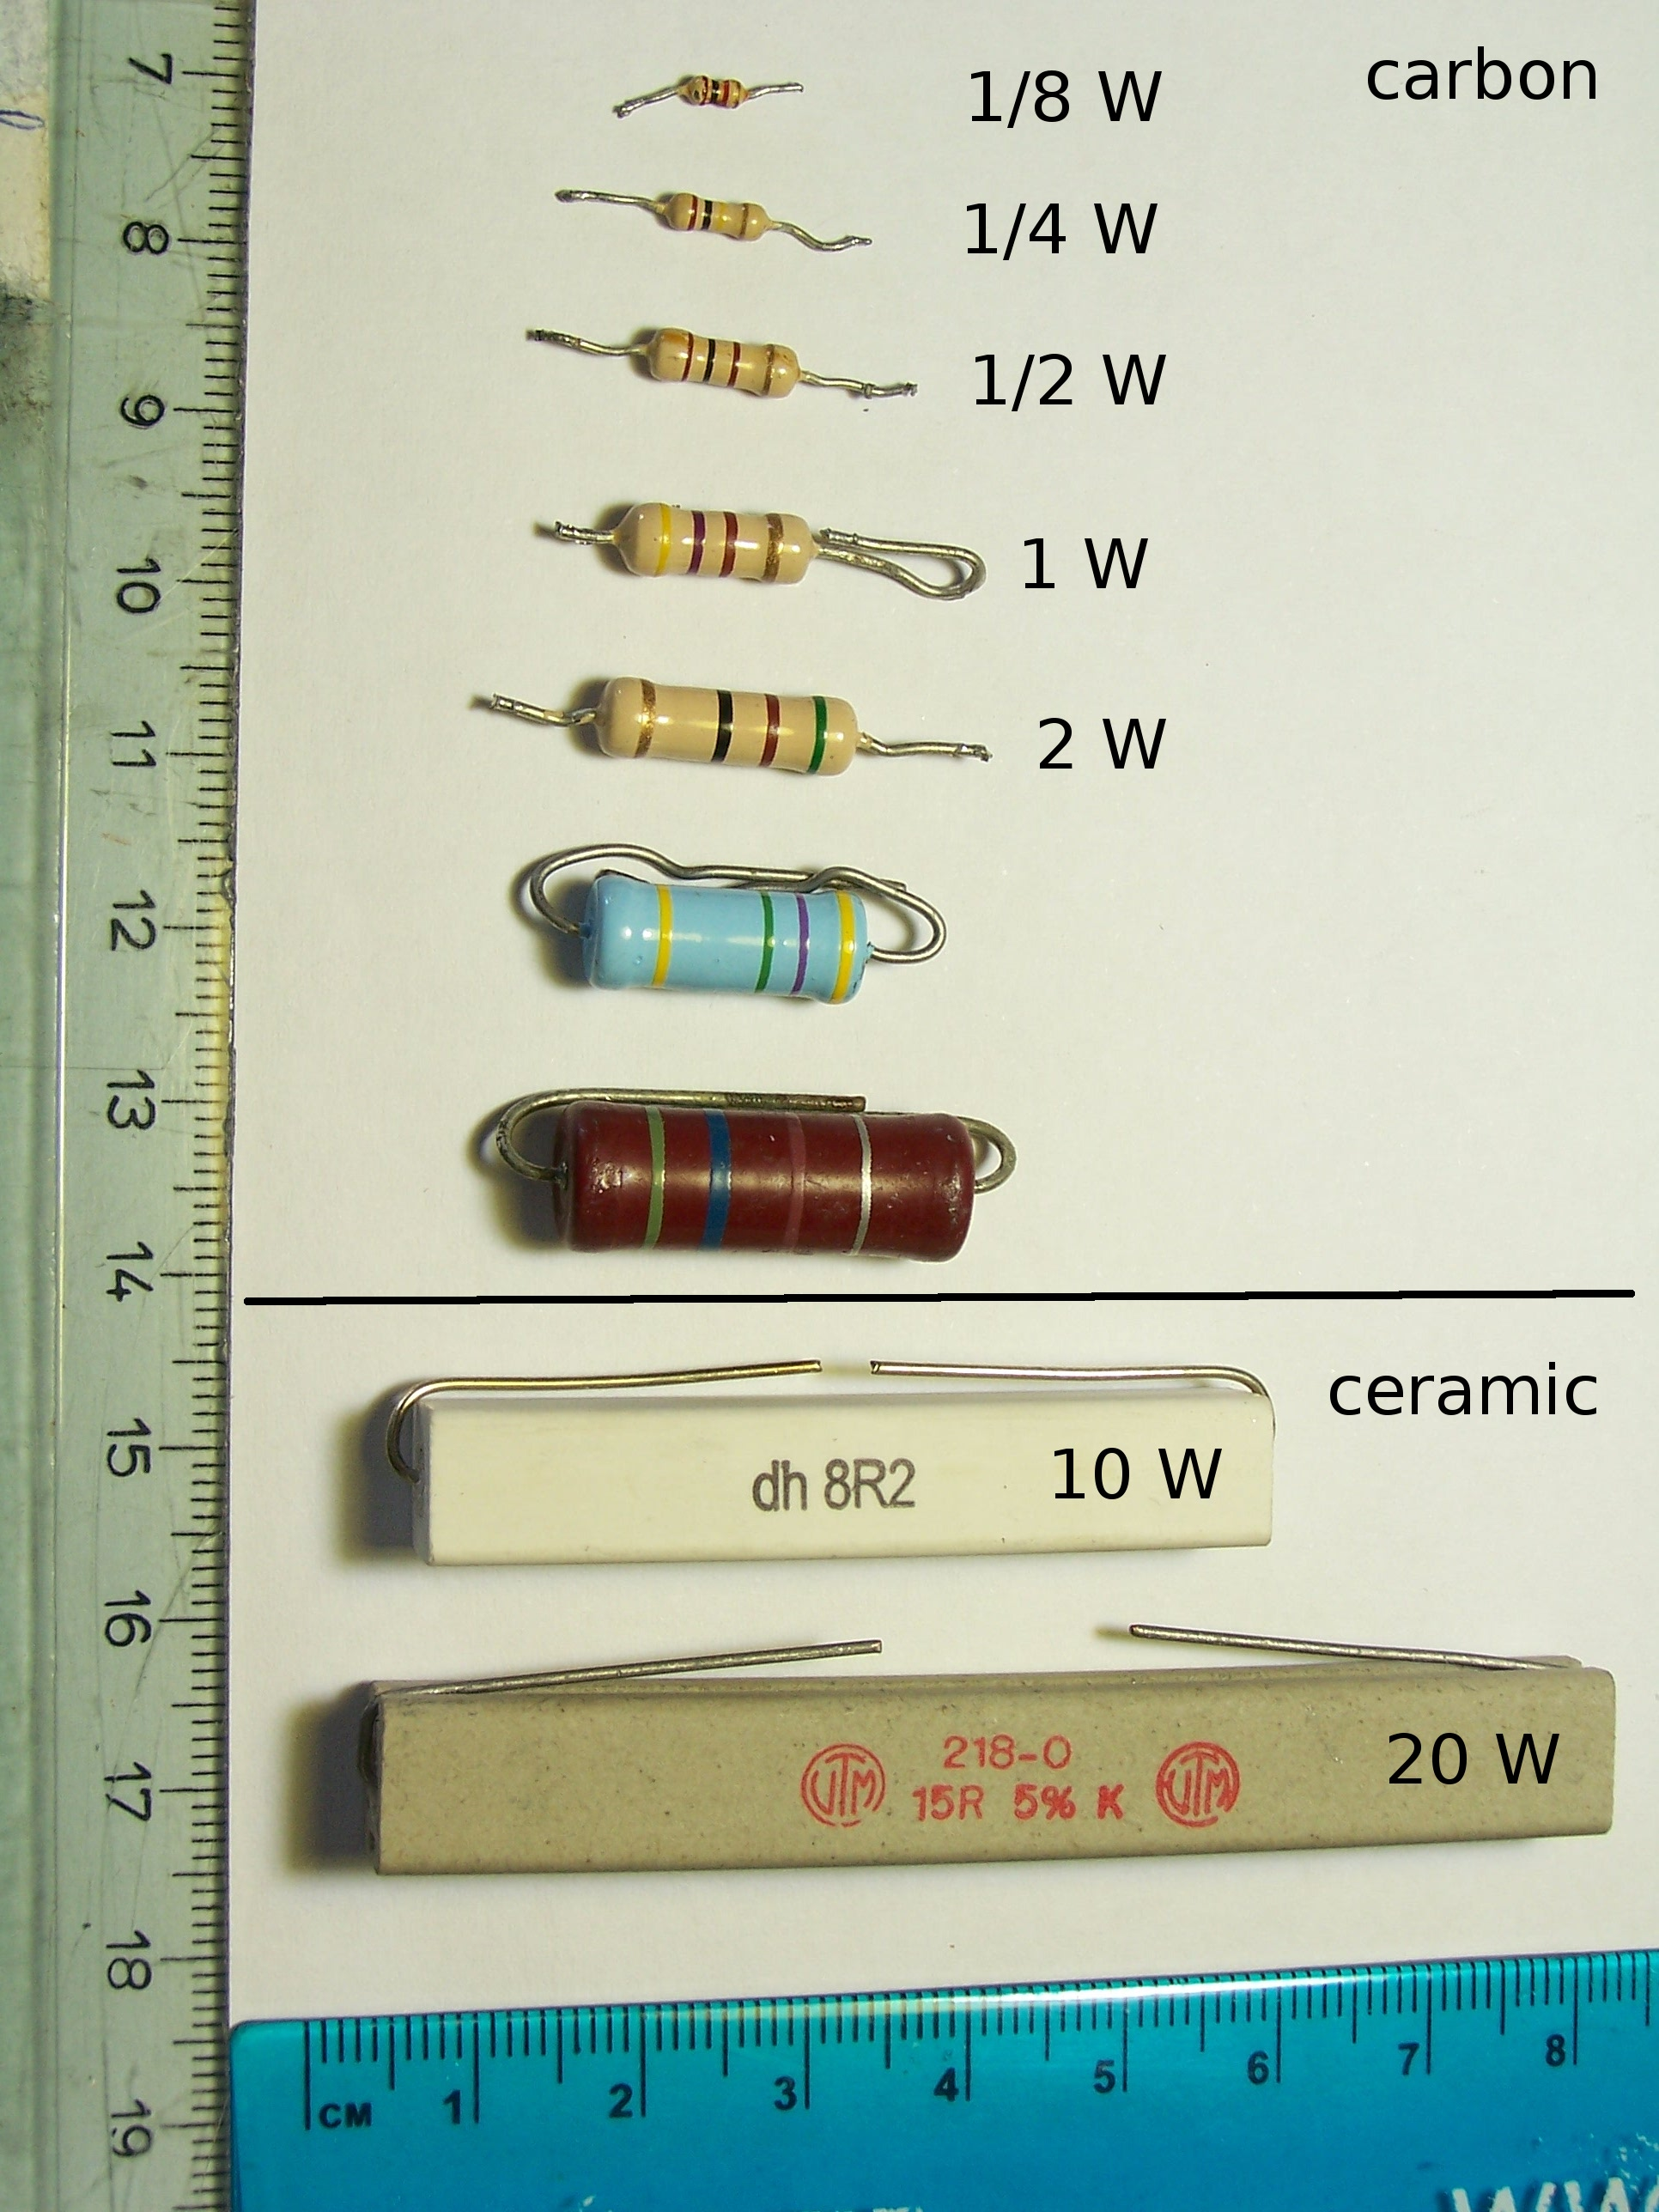
\includegraphics[width=0.35\textwidth]{laborator_01/figuri/7_resistors_power_ratings}
	\caption{Rezistoare -- puteri maxim admise \cite{rezistoare_puteri}.}
	\label{fig:rezistoare_puteri}
\end{figure}

Rela'tia \ref{eq:sarcina} arat'a c'a tensiunea de ie'sire nu este afectat'a de sarcin'a dac'a rezisten'ta de sarcin'a $R_s$ este mult mai mare decat $R_2$, sau altfel spus, dac'a $R_2 \ll R_s$. Dac'a $R_s$ este impus'a 'si cunoscut'a, atunci e indicat s'a alegem $R_2$ ('si implicit $R_1$ 'in func'tie de raportul $\alpha$ dorit) c\^at mai mic'a. 
%raportat'a la rezisten'ta de sarcin'a (de exemplu de 100 de ori mai mic'a).

\begin{retine}
Valori mici ale rezisten'telor $R_1$ 'si $R_2$ cresc precizia circuitului divizor de tensiune.
\end{retine}

Pe de alt'a parte, cu c\^at alegem rezisten'tele $R_1$ 'si $R_2$ mai mici, cu at\^at curentul care le str'abate este mai mare. Asta 'inseamn'a c'a puterea consumat'a de c'atre rezisten'te $P = RI^2$ va fi mai mare, deci ele se vor 'inc'alzi mai mult 'si se pot distruge. Dimensiunea rezistoarelor arat'a maximul de putere care e disipat'a 'inainte ca temperatura s'a creasc'a excesiv de mult (Fig. \ref{fig:rezistoare_puteri}).

\begin{retine}
Valori mari ale rezisten'telor $R_1$ 'si $R_2$ scad curentul deci 'si puterea consumat'a.
\end{retine}

\begin{exercise}
Determina'ti curentul maxim care poate str'abate un rezistor cu rezisten'ta de $180~\Omega$ 'si o putere maxim'a admis'a de 0.25 W. 
\end{exercise}

'In alegerea valorilor rezisten'telor trebuie c'autat echilibrul 'intre precizie 'si putere consumat'a. 

\begin{exercise}
Proiecta'ti un divizor de tensiune cu 4, care va fi alimentat cu o tensiune de $8$ V, conform Fig. \ref{fig:7_exercitiul1}. Rezisten'tele folosite au o putere maxim'a admis'a de $0.25$ W.
\end{exercise}

\begin{figure}[!t]
	\centering
		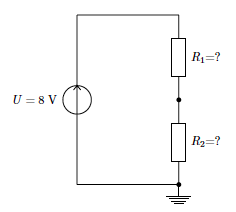
\includegraphics[width=0.5\textwidth]{laborator_01/figuri/7_exercitiul1}
	\caption{Proiectarea unui divizor de tensiune cu 4. Rezisten'tele au o putere maxim'a admis'a de 0.25 W.}
	\label{fig:7_exercitiul1}
\end{figure}